
\section{maincontent}

\begin{frame}
\frametitle{Strong-Field Ionization Phenomena Revealed by Quantum Trajectories \\
\small (Phys. Rev. Lett. \textbf{133}, 073201 (2024))}
\framesubtitle{Laser-atom interaction in Strong field}


\footnotesize
%\begin{textblock*}{200pt}(250pt,60pt)
%\begin{itemize}
%\item 3 steps model
%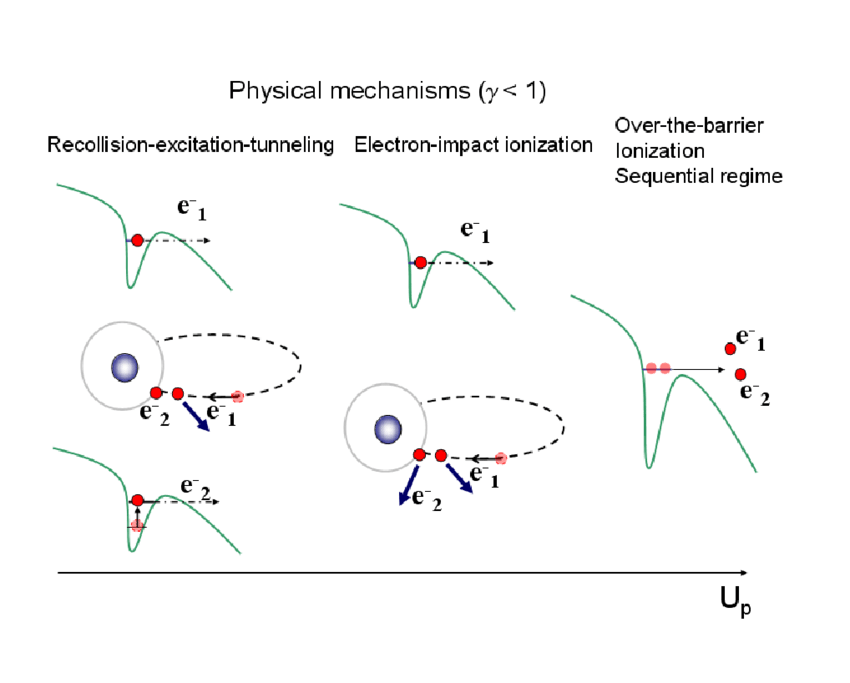
\includegraphics[scale=.20]{images/Color-online-Schematic-representation-of-the-dominant-physical-mechanisms-behind.png}
%\end{itemize}
%\end{textblock*}
 
\begin{textblock*}{400pt}(30pt,60pt)
\begin{itemize}
\footnotesize
\item The Keldysh parameter
%%
\includegraphics[scale=.75]{images/polcls.png}
\begin{align}
\begin{split}
 \gamma_K \equiv \omega\sqrt{2I_p}/E_0
\end{split}
 \nonumber 
\end{align}
$\gamma_k < 1 \longrightarrow \mbox{ Tunnel ionization (horizontal channel)}$ \\
$\gamma_k > 1 \longrightarrow \mbox{ Tunnel ionization (vertical channel)}$ \\
$\gamma_k \sim 1 \longrightarrow \mbox{ Intermediate regime}$ 

\begin{itemize}
\footnotesize
 \item[$\bullet$] Provides a quantitative understanding of the dominant
photoionization mechanism
\end{itemize}
\begin{itemize}
\footnotesize
 \item[$\bullet$] Disregards the nature of the binding potential
and excited state
 \item[$\bullet$] Reduces the intricacies of the field to the field strength
only
 \item[$\bullet$] Wrongly assume that the tunneling wavepacket 
always start in the classically allowed region
 \item[$\bullet$] Over the barrier ionization (OBI) is poorly rendered
\end{itemize}
\vspace{10pt}
\item Since the dynamics of the electron becomes classical, 
trajectories based approaches are appropriate 
\vspace{15pt}
\item \textbf{This paper attempts at proposing a more suitable parameters
than $\gamma_K$ for describing the interaction}

\end{itemize}
\end{textblock*}


%\begin{textblock*}{100pt}(330pt,210pt)
%\begin{align}
%\footnotesize
%U_p = \frac{F_0^2}{4\omega^2}, \hspace{20pt} 
%\gamma = \sqrt{\frac{I_p}{2U_p}}\nonumber
%\end{align}
%\end{textblock*}

\end{frame}



\begin{frame}
\frametitle{Strong-Field Ionization Phenomena Revealed by Quantum Trajectories \\
\small (Phys. Rev. Lett. \textbf{133}, 073201 (2024))}
\framesubtitle{The de Broglie-Bohm quantum theory}


\footnotesize
%\begin{textblock*}{200pt}(250pt,60pt)
%\begin{itemize}
%\item 3 steps model
%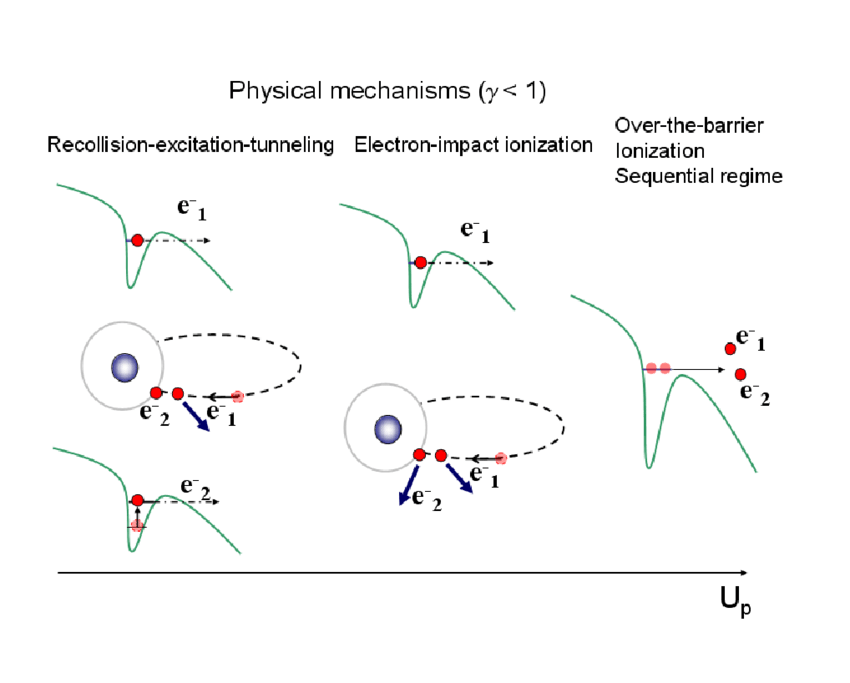
\includegraphics[scale=.20]{images/Color-online-Schematic-representation-of-the-dominant-physical-mechanisms-behind.png}
%\end{itemize}
%\end{textblock*}
 
\begin{textblock*}{400pt}(30pt,60pt)
Trajectories are researched by solving the TDSE, first
\begin{align}
\begin{split}
 i\frac{d}{dt}\Psi(t) = H(t)\Psi(t), 
   \hspace{20pt} H(t) & = H_0 - \boldsymbol{p}\boldsymbol{A}(t),
\end{split}
 \nonumber \\
\begin{split}
\boldsymbol{E}(t) = -\frac{d}{dt}\boldsymbol{A}(t), \hspace{20pt}
\boldsymbol{A}(t) &= -A_0 \cos^4\left(\frac{\pi t}{NT}\right)\sin (\omega t)\boldsymbol{\hat{x}}, \hspace{20pt}
 t \in \left[ -NT/2, NT/2 \right], \hspace{20pt} T = 2\pi/\omega
\end{split} \nonumber
\end{align}
\begin{itemize}
\item Bohmian formalism and quantum potential
\begin{align}
 i\frac{\partial \psi}{\partial t} = \Bigg( -\frac{1}{2}\nabla^2 + V\Bigg)\psi,
\hspace{10pt} \mbox{ with } \hspace{10pt} \psi = R\exp(iS), 
\hspace{20pt} 
\rho(\boldsymbol{r},t) = \left| \psi(\boldsymbol{r},t)\right|^2\nonumber
\end{align}
Using the above expression of the wavefunction $\psi$ in the 
Schr\"odinger equation, and considering only the real part 
leaves us with 
\begin{align}
 \frac{\partial S}{\partial t} = -\frac{1}{2}(\nabla S)^2 
          + \frac{1}{2}\Bigg( \frac{\nabla^2 R}{R} \Bigg) - V \nonumber
\end{align}

\end{itemize}
\end{textblock*}


\begin{textblock*}{400pt}(200pt,210pt)
\begin{align}
Q = -\frac{1}{2} \rho^{-1/2} \nabla^2 \rho^{1/2}
\end{align}
\end{textblock*}



\end{frame}


\begin{frame}
\frametitle{Strong-Field Ionization Phenomena Revealed by Quantum Trajectories \\
\small (Phys. Rev. Lett. \textbf{133}, 073201 (2024))}
\framesubtitle{Bohmian theory - Velocity field and trajectories}


\footnotesize
%\begin{textblock*}{200pt}(250pt,60pt)
%\begin{itemize}
%\item 3 steps model
%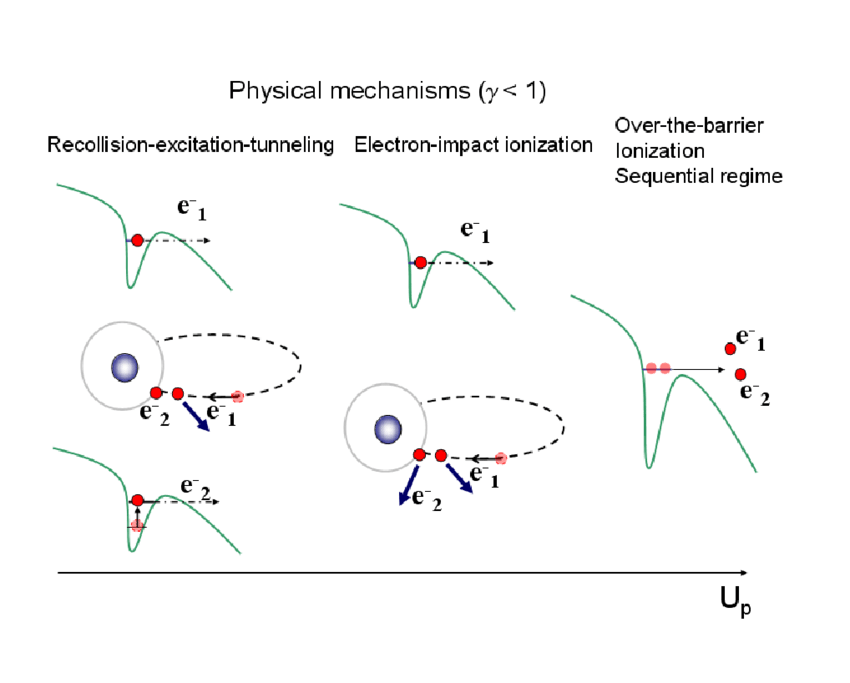
\includegraphics[scale=.20]{images/Color-online-Schematic-representation-of-the-dominant-physical-mechanisms-behind.png}
%\end{itemize}
%\end{textblock*}
 
\begin{textblock*}{400pt}(30pt,60pt)
\footnotesize
\begin{itemize}
\item In the Bohmian formalism, velocity is given by
\begin{align}
\begin{split}
 \boldsymbol{v}(\boldsymbol{r},t) 
   = \boldsymbol{j}(\boldsymbol{r},t) /  \rho(\boldsymbol{r},t), 
\hspace{20pt} 
\boldsymbol{j}(\boldsymbol{r},t) = Re\Bigg(\Psi^*(\boldsymbol{r},t)
\left( -i\Delta + \boldsymbol{A}(t)  \right) \Psi(\boldsymbol{r},t)\Bigg)
\nonumber
\end{split}
\end{align}
\begin{itemize}
\footnotesize
\item[$\bullet$] Retrieving $\psi$ from the TDSE
\item[$\bullet$] Propagation of the trajectories from different positions 
$\boldsymbol{r}_0$
\item[$\bullet$] Reconstruction of the wavefunction from the trajectories
at any given time
\end{itemize}
\item Computation of time and radii exit $t_{\rm ex}$ and $r_{\rm ex}$
from the condition
\begin{align}
\Delta \mathcal{E}(t_{\rm ex}) = 0, \hspace{20pt}
\Delta \mathcal{E}(t) = v^2(t)/2  + Q(t), \hspace{20pt} \nonumber
\end{align}
where  $\Delta \mathcal{E}(t)$ is the difference between the energy of 
the trajectory $\mathcal{E}(t)$ and $I_p$
\item The quantum potential $Q(t)$ is responsible for all quantum effects and the nonzero velocity at the exit 
\vspace{10pt}
\item In the classical limit 
\begin{align}
Q(t) \longrightarrow 0 \nonumber
\end{align}
\end{itemize}
\end{textblock*}




\end{frame}





\begin{frame}
\frametitle{Strong-Field Ionization Phenomena Revealed by Quantum Trajectories \\
\small (Phys. Rev. Lett. \textbf{133}, 073201 (2024))}
\framesubtitle{The tunneling parameter}

\small

\begin{textblock*}{100pt}(280pt,100pt)
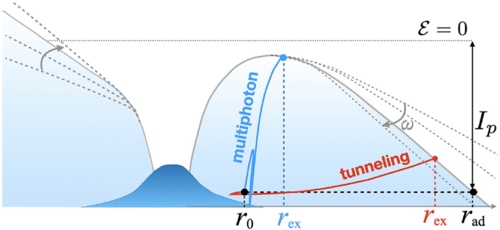
\includegraphics[scale=.34]{images/medium.png}
\end{textblock*}

\begin{textblock*}{250pt}(30pt,60pt)
\begin{align}
\beta\left( \boldsymbol{r}_0\right) \equiv 
\frac{r_{\rm ex}\left( \boldsymbol{r}_0\right) - r_0}
      {r_{\rm ad}\left( \boldsymbol{r}_0\right) - r_0} \nonumber
\end{align}
\begin{itemize}
\footnotesize
\item $0 \leqslant \beta \leqslant 1$ quantifies the degree of tunneling
for a trajectory starting at $r_0$
\item For vertical ionization, $r_{\rm ex} = r_0 \longrightarrow \beta = 0$
\item For horizontal ionization, 
$r_{\rm ex} = r_{\rm ad} \longrightarrow \beta = 1$
\item $\beta$ aslo exists in the eventuality that 
$r_{\rm ex} \geqslant r_{\rm ad}$ (OBI...)
\vspace{20pt}
\item The adiabatic radius $r_{\rm ad}$ corresponds to a trajectory such as 
$\mathcal{E} = -I_p $
\end{itemize}
\end{textblock*}


\end{frame}

%
%
\begin{frame}
\frametitle{Strong-Field Ionization Phenomena Revealed by Quantum Trajectories \\
\small (Phys. Rev. Lett. \textbf{133}, 073201 (2024))}
\framesubtitle{Photoionization of atomic hydrogen as a function of $r_0$}

\begin{textblock*}{100pt}(300pt,70pt)

\includegraphics[scale=.33, trim={0 0 0 0}, clip]{images/medium1.png}
\end{textblock*}

\small
\begin{textblock*}{250pt}(30pt,60pt)
\begin{itemize}
\footnotesize
\item 2 dimensional plot of $\beta(\boldsymbol{r}_0)$ as a function of $r_0$
in the $xy-$plane
\item 2 different pulses describing MPI and TI are used
\item Fig. 2(b) provides additional details on the dynamics of the ionization
\begin{itemize}
\footnotesize
\item[$\bullet$] Tunnel ionization dominates in the direction longitudinal 
to the field past a certain $r_0$  
\item[$\bullet$] Multiphoton mechanism occurs in the direction 
transversal to the field  ionization
\item[$\bullet$] At large distances, the mechanism naturally exhibits 
a multiphoton character
\end{itemize}
\vspace{30pt}
\begin{align}
\beta & \longrightarrow 0    \hspace{30pt} \mbox{vertical channel} \nonumber\\
\beta & \longrightarrow 1    \hspace{30pt} \mbox{horizontal channel} \nonumber
\end{align}
\end{itemize}
\end{textblock*}



\end{frame}


\begin{frame}
\frametitle{Strong-Field Ionization Phenomena Revealed by Quantum Trajectories \\
\small (Phys. Rev. Lett. \textbf{133}, 073201 (2024))}
\framesubtitle{Quantum adiabatic parameter}

\small
\begin{textblock*}{400pt}(30pt,60pt)
\begin{itemize}
\footnotesize
\item Statistically averaged tunneling level of the ionization process
\begin{align}
\bar{\beta} = W_0^{-1} \int_{\mathcal D} \beta\left( \boldsymbol{r}_0\right)
\rho\left( \boldsymbol{r}_0,0\right)
d^3 \boldsymbol{r}_0 \nonumber
\end{align}
\begin{itemize}
\footnotesize
\item[$\bullet$] $\mathcal{D}$ denotes the set of ionizing trajectories
\item[$\bullet$] $W_0 = \int_{\mathcal D} \rho\left(\boldsymbol{r}_0,0\right)d^3\boldsymbol{r}_0$ is the total ionization probability
\end{itemize}

\vspace{10pt}

\item To compare with the Keldysh parameter $\gamma_K$, they define 
the quantum adiabatic parameter $\gamma_q$

\begin{align}
\gamma_q \equiv \frac{1-\bar{\beta}}{\bar{\beta}}  \nonumber
\end{align}
\begin{itemize}
\footnotesize
\item[$\bullet$] This quantity has the same limits and meaning as $\gamma_K$
\item[$\bullet$] $\gamma_q \longrightarrow 0$ for TI and
$\gamma_q \longrightarrow \infty$ for MPI
\end{itemize}
\end{itemize}

\end{textblock*}

\end{frame}


%\begin{frame}
%\frametitle{Strong-Field Ionization Phenomena Revealed by Quantum Trajectories \\
%\small (Phys. Rev. Lett. \textbf{133}, 073201 (2024))}
%\framesubtitle{What to expect from this paper}
%
%\small
%\begin{textblock*}{400pt}(30pt,60pt)
%\begin{itemize}
%\item Few studies to date have explored the how CEP affects 
%bound-state populations
%\item CEP can be used to clearly determine when the dynamic changed from 
%Multiphoton- (MP) to tunneling-ionization plus recapture (FTI)
%\vspace{10pt}
%\item In this paper, the followings are done
%\begin{itemize}
%\footnotesize
%\item[$\bullet$] Experimental investigation of excitation rates of $\rm Ar$
%as a function of CEP in the tunneling regime
%\item[$\bullet$] Showing that bound-state populations dependence on CEP 
%is strong in the tunneling regime
%\item[$\bullet$] Showing at which instant between MP and tunneling regimes,
%dynamics changes
%\end{itemize}
%\end{itemize}
%
%\end{textblock*}
%
%\end{frame}





 
 
\begin{frame}
\frametitle{Strong-Field Ionization Phenomena Revealed by Quantum Trajectories \\
\small (Phys. Rev. Lett. \textbf{133}, 073201 (2024))}
\framesubtitle{Quantum adiabatic parameter as a function of the intensity}

\begin{textblock*}{100pt}(60pt,60pt)

\includegraphics[scale=.55]{images/medium2.png}
\end{textblock*}

\small
\begin{textblock*}{400pt}(30pt,150pt)
\begin{itemize}
\footnotesize
\item Fig.3(a) Comparison of $\gamma_q$ for 2 different potentials 
with $\gamma_K$ for different intensities
\begin{itemize}
\footnotesize
\item[$\bullet$] For weak fields, MPI is more pronounced than predicted 
by the Keldysh approximation
\item[$\bullet$] The difference between the potentials 
is sharp at low intensities. $\gamma_q$ is more sensitive than $\gamma_K$
\end{itemize}
\item Fig. 3(b) Comparison of $\gamma_q$ for different pulse duration
\begin{itemize}
\footnotesize
\item[$\bullet$] 4 cycles has more enhanced MPI and TI mechanisms because 
more laser peaks 
\end{itemize}
\item Fig. 3(c) Comparison of $\gamma_q$ for different wavelengths
\begin{itemize}
\footnotesize
\item[$\bullet$] The results agree with general prediction 
\end{itemize}
\end{itemize}
\end{textblock*}


\end{frame}




\begin{frame}
\frametitle{Strong-Field Ionization Phenomena Revealed by Quantum Trajectories \\
\small (Phys. Rev. Lett. \textbf{133}, 073201 (2024))}

\framesubtitle{Quantum adiabatic parameter as a function of the frequency}

\begin{textblock*}{100pt}(280pt,70pt)

\includegraphics[scale=.33]{images/medium3.png}
\end{textblock*}

\small
\begin{textblock*}{250pt}(30pt,60pt)
\begin{itemize}
\footnotesize
%\item The number of optical cylces is 2
\item Fig. 4(a) Intermittent steps at which $\gamma_q$ ceases to progress 
uniformily are observed 
\begin{itemize}
\footnotesize
\item[$\bullet$] Correspond to channel closings known to suppress ionization
\end{itemize}
\vspace{10pt}
\item Fig. 4(b) Results for 2 photon ionization in the $2s$ state
\begin{itemize}
\footnotesize
\item[$\bullet$] Sharp drop near resonnance indicating
a preference for TI in this frequency region
\item[$\bullet$] Population transfer to the $3p$ state favoring TI 
\vspace{5pt}
\item[$\bullet$] The point is that it reproduces a specific behaviour 
reported in the litterature\footnote{\Tiny K. Mishima \textit{et al.}, Phys. Rev. A 66, 033401 (2022)} 
\end{itemize}
\end{itemize}
\end{textblock*}

\end{frame}




\begin{frame}
\frametitle{Strong-Field Ionization Phenomena Revealed by Quantum Trajectories \\
\small (Phys. Rev. Lett. \textbf{133}, 073201 (2024))}

\framesubtitle{Over the barrier ionization}

\begin{textblock*}{100pt}(280pt,70pt)

\includegraphics[scale=.30]{images/medium4.png}
\end{textblock*}

\small
\begin{textblock*}{250pt}(30pt,60pt)
\begin{itemize}
\footnotesize
\item OBI happens if either $\mathcal{E}(t)$ remains above the barrier
or $\mathcal{E}(t_{\rm ex}) \leqslant I_p$ 
\item Going by this definition, Fig. 5 compares $W_0$ and $W_{\rm OBI}$ 
for different intensities 
\begin{itemize}
\footnotesize
\item[$\bullet$] $W_{\rm OBI}$ experiences a sharp increase when
the top of the barrier becomes lower than $I_p$
\item[$\bullet$] Subsequentially, the increase rate is similar to $W_0$
\end{itemize}
\item At intensities about 10 times higher than the OBI limit, a steady state is reached where $W_{\rm OBI}/W_0 \sim 0.6$
\end{itemize}
\end{textblock*}

\end{frame}


